\chapter{工欲善其事,必先利其器}
\label{cha:pre-requisite}

用\LaTeX{}撰写毕业论文是一件赏心乐事,前提是你得会。网上关于\LaTeX{}的入门教程很多,下面这
几个就很不错,花一两天时间去熟悉一下,

\begin{enumerate}
\item \LaTeX{} on Wikibooks\footnote{\url{https://en.wikibooks.org/wiki/LaTeX}}
\item The very short guide to typesetting with
  \LaTeX{}\footnote{\url{http://tug.ctan.org/info/latex-veryshortguide/veryshortguide.pdf}}
\item The not so Short Introduction to
  \LaTeX{}\footnote{\url{https://www.ctan.org/tex-archive/info/lshort/english/?lang=en}}
\end{enumerate}
有了对\LaTeX{}的基础认识之后,再接着往下看。

\section{工作环境}
\label{sec:env}

工作环境当然要清静、优雅。一杯热咖啡,配上轻音乐……除此之外,你还需要一
台电脑,最好是像我用的电脑。硬件不用太高级,但内存最好大一些,不少
于4G为宜,因为在我看,CPU已经足够快了,电脑运行是否顺畅,更多的是取决于
内存是否充足。下面简单介绍一下我们需要的软件环境和工具。

\subsection{操作系统}

我用Debian GNU/Linux ()%
\footnote{: \url{https://en.wikipedia.org/wiki/Debian}}的测试
(testing)版。为什么不用MS Windows? 因为~\ldots 当然不是它不好,而是我缺乏
足够的耐心。我的Debian系统从来不考验我的耐心。
很久以前,好像是2017年,在\href{https://www.zhihu.com}{知乎}上曾经看到
过一个问题 --- 不做开发的话,Linux是否适合日常使用?看到这个问题,我的第
一反应就是,“日常使用”这个词太含糊了。随后,我又意识到,如果认为“日常使
用”这个词不够具体,那么我就是在或多或少地承认“Linux不适合所有的日用场
景”。做为一个Debian铁杆用户,忽然发现“Linux不适合所有的日用场景”,这实
在令我有点沮丧。没错,我从1998年开始接触Debian,之后我所有的办公、私人
电脑上都只有Debian这一个系统。而且,我不是开发者。虽然我的确有一个计算
机专业的硕士学历,但十几年来,除了“Hello, world!”之外,我几乎什么程序都
没写过。我之所以写“Hello, world!”也完全是出于最基础的教学需要。我在大学
里教《Linux应用基础》和《操作系统原理》,讲到开发的时候,好歹得举个简单
的例子嘛。一个教计算机的老师不搞开发,我知道,这很不……。但是,做为一个
懒人,我也有我懒的借口。在天朝搞开发、搞科研,在我看就是“恭喜发财!”。
如果没有经济上的困扰,我觉得把时间兑换成钞票是相当不划算的事情。所以,
当我不得不对人家坦白说“我在事业上一事无成”的时候,我通常会向人家展示一
下我寒暑假的骑行游记\footnote{https://cs6.swfu.edu.cn/~wx672/travelogs},%
以此证明我这些年也没白活。否则,后面的聊天……反正我不觉得尴尬,
尴尬的就是别人。不管怎么说,我就是一个地地道道的Linux日常使用者,而且不搞开发,
而且我的Debian能满足我几乎所有的日常需求。当然,我的日常需求也的确相当
简单(上网、听歌、看片、写讲义、做幻灯片……)。

那么,Linux到底能不能应付所有的“日常使用”场景?我觉得,能,但你很难用某
一个通用的(默认安装配置的)Linux系统来满足所有的场景。通常,你要对自己
的系统做有针对性的配置,从而让它能够满足你的特定日常使用需求。与此相对
比,MAC OSX基本上做到了用一个系统来满足所有的用户需求,无需“私人订制”,
这的确是它的优势所在。但“私人定制”的确也是个诱人的字眼,不是吗?

那么,哪个Linux品牌(发行版)最好用?严肃地说,都一样好用。不信?在十
台电脑上装十个牌子的Linux,放到你面前,你会发现的确都很好用,也很漂亮,
而且你分辨不出谁是谁。换句话说,做为普通用户,你不必关心“牌子”问题,因
为各品牌的不同之处不在于使用,而在于管理。Debian和Redhat的系统管理方
式(操作命令、配置文件的格式等等)是大不相同的。而“管理”是管理员的事情,
做为一个普通用户的确不需要去操心。如果你想成为一个管理员,你至少得先成
为一个熟练用户才行吧。

那么,如果我打定主意要用Linux了,我该装哪个牌子的系统?我觉得,你周围的
熟练用户都用什么牌子,你就跟着用什么牌子。很显然,这样你能最方便地获得
帮助。如果你周围没有熟练用户,那么我建议你用Debian,因为它稳定性
好,bug少,软件库最大,社区最大,管理(软件包的安装、卸载、升级)方式简
单。下面简单罗列一下我在Linux平台不能顺利完成的事情:

\begin{itemize}
\item \href{https://im.dingtalk.com}{Dingtalk的网页版}似乎永久性地进入
  了“系统维护中”,为此,我尝试了WINE\footnote{https://wiki.winehq.org/Debian},%
  也尝试了在Virtualbox虚拟机里装
  个Android-x86\footnote{https://www.android-x86.org/},%
  两个办法都行得通,但总感觉代价偏高。WINE和Virtualbox都很优秀,问题出
  在钉钉上,它不仅臃肿,而且buggy,我实在没心情伺候它。还好,折腾了一
  年多之后,钉钉终于有了Linux版,虽然还是很臃肿、很buggy,但总算能对付
  着用了。
  % 所以我目前的解决
  % 方案是:1)如果想借用电脑的实体键盘快速打字的话,我就用scrcpy%
  % \footnote{https://github.com/Genymobile/scrcpy};2)如果想在电脑与手
  % 机之间快速传输文件,我就用qrcp%
  % \footnote{https://github.com/claudiodangelis/qrcp}。
\item Linux平台没有原生的炒股软件,但通过WINE也还可以挺顺畅地应付。
\end{itemize}

除此之外,我的Debian就只剩下优点了。当然,对于一个传统的Windows用户,
他要面对的困扰远不止这么两条,比如说,

\begin{itemize}
\item 他习惯于使用MS-Office做事情(可以尝试Libreoffice,或者WPS)
\item 他要玩游戏(也许可以WINE)
\item 他要QQ
\item 他要微信
\item 他要……
\end{itemize}


总之,做为入门用户,而且被Windows/QQ/Wechat/Baidu/360用户群包围着
\footnote{腾讯已经发布了QQ和微信的Linux版本,据说还不错。},又生
活在防火长城之下……困难总会有的,但并非无法克服。Debian可能是我人生中最
正确的一个选择了,干净,自由。

\subsection{桌面环境}

Linux社区流传着一句古老的元旦玩笑 --- “今年将是the year of Linux
desktop”。为了这一梦想,Linux的各个品牌都热衷于以华丽的桌面环境为诱饵,
招揽Windows用户。兄弟我年轻的时候,也是“重色思倾国”,和各种花容月貌的桌
面环境迷醉缠绵。后来发现,的确都很漂亮,但漂亮的东西都不便宜。一套完整
的Gnome或者KDE要安装数百个大大小小的软件包,占用数百兆硬盘,数百兆内存,
为系统增加数不清的bug,每次系统更新都要占用更多的带宽,花费更长的时间……而
这一切代价,只是为了“漂亮”和“方便”。

“漂亮”和“方便”当然是好事情,但它们是两个相当主观的词。“漂亮”很主观,情
人眼里出西施,母猪也能赛貂蝉,漂亮不漂亮的,基本上取决于你当时荷尔蒙的
高低,高兴就好。“方便”也很主观,我们身边的绝大多数电脑用户都是离不开鼠标的,因为它方便。但Emacs%
\footnote{: \url{https://www.gnu.org/software/emacs/}}或者Vim%
\footnote{: \url{https://www.vim.org/}}的粉丝们基本上完全抛开了鼠标,这
也是因为方便。对于Windows用户,抛开鼠标就像病人抛开拐杖一样痛苦。但只有
不依赖于拐杖的人才是健康的,不是吗?所以,怎么才算是方便呢,作为计科专
业的学生,你不该斟酌一下吗?

写毕业论文的话,我们完全不需要昂贵的桌面环境,有个便宜的window
manager就足够了。前面刚忏悔过,年轻的我是个desktop-hopper,在眼花
缭乱的桌面环境间换来跳去。“十年一觉扬州梦”,如今眼睛也花了,胡子也白
了,“再回首,……,才知道平平淡淡从从容容才是真”,于是
我返璞归真,由 desktop-hopper 变异为 WM-hopper。先用了十多年Sawfish%
\footnote{\url{https://en.wikipedia.org/wiki/Sawfish_(window_manager)}}
,Sawfish曾经是Gnome默认的窗口管理器,它界面足够的简单,功能足够的丰富,
配置足够的容易。而且和Emacs一样,它也是用Lisp写成的,算是Emacs的近亲吧。
这是我偏爱Sawfish的一个重要原因。后来,Sawfish老不更新,我就见异思迁,
另觅新欢,找了yet another Lisp-based tiling window manager ---
stumpwm\footnote{\url{https://stumpwm.github.io/}}。一直想好好学学Lisp,
无奈拖延症晚期了……又一变异,就躺平了。

近两年我都在用DWM\footnote{\url{https://dwm.suckless.org/}},一个很不
错的平铺式窗口管理器(tiling window manager%
\footnote{\url{https://en.wikipedia.org/wiki/Tiling_window_manager}})。%
它可以自动让所有的窗口互不重叠地铺满整个屏幕,非常适合大屏幕。%
而且dwm支持全键盘操作,有了它,你可以完全忘掉鼠标的存在。另外,作为一个
计科专业的学生,我觉得好歹你要做过一两个软件项目,才好意思写论文
吧。DWM就是个很小巧的C编程项目,代码量很少,易于学习。通过修改配置文件
就可以积累一些C编程的实战经验,何乐而不为?

\subsection{必备软件}

除了窗口管理器,显然你还需要几个“窗口”。下面这三个恐怕是必须有的:

\begin{description}
\item[Web浏览器] 原来我用Chromium\footnote{%
    : \url{https://en.wikipedia.org/wiki/Chromium_(web_browser)}},2019年
  初开始,改用Qutebrowser \footnote{%
    \qutebrowser{}: \url{https://en.wikipedia.org/wiki/Qutebrowser}} ,因为它小、快、灵、
  省内存、支持全键盘操作;
\item[PDF阅读工具] 我用Emacs的pdf-tools插件。在Emacs里,可以在一
  个buffer里写\TeX{},在另一个buffer里看PDF。还可以很方便地在两个buffer中
  对应的位置跳来跳去;
\item[终端] 我用st\footnote{\url{https://st.suckless.org/}}。其实,终端
  软件都差不多,有一个就行。真正不可或缺的
  是tmux\footnote{\url{https://en.wikipedia.org/wiki/Tmux}},有了它,一
  个终端可以当一万个用。
\end{description}

除了“窗口”之外,你还需要:
\begin{description}
\item[\LaTeX{}套件:]
  TeXLive\footnote{\url{https://en.wikipedia.org/wiki/TeX_Live}},它完
  备而庞大,但如果就是写个科技论文,我们只需要其中很少的一些软件包就够
  了。附录\ref{app:pkg}中列出了参照本教程写论文所需的所有软件包,可供参
  考。
\item[中文字体:] 完全不必操心,因为TeXLive有很好的中文支持。如果抛
  开\TeX{}不谈,就日常使用而言,我比较喜欢Noto字体\footnote{%
    \url{https://en.wikipedia.org/wiki/Noto_fonts}}。它是Google推出的开
  源字体。Debian库里自带,装上就好。所谓“Noto”就是Notofu的意思,也就是
  说Noto字体的终极目标是消灭所有的豆腐块(缺字)。Noto有专门的CJK字体包,
  只是尚缺楷体。楷体我用Debian库里自带的arphic-ukai,它是台湾文鼎科技\footnote{%
    \url{https://en.wikipedia.org/wiki/Arphic_Technology}}推出的开源字
  体。你当然也可以选用Windows字体,只要从你的Windows系统里拷贝过来就行
  了。这也许是你人生中唯一需要Windows的时候。
\end{description}

\subsection{编辑器}
\label{sec:emacs}

Emacs()是世界上最强大的编辑器\cite{emacs},没有之一。作为计科专业的
学生,如果你不熟悉它的使用,怎么好意思写毕业论文呢?我从1997年开始接
触Emacs,至今已经27年了。我不是程序员,从来就不是,但是,I love Emacs!
1997年的时候,还没有你今天见到的这么多IDE\footnote{%
  集成开发环境(Integrated Development Environment)。},所以Emacs就是
当年最好的IDE。25年来,虽然我既没有搞开发,也没为Emacs贡献任何插件,但
我还是从Emacs获得了巨大的乐趣。直到今天,在我看,Emacs还是最好的IDE。不
信?我们先看看什么是IDE。一个IDE无非包括如下一些功能模块:一个编辑器,
一个编译器,一个调试器,和其他一些辅助功能,比如用鼠标拖控件。什么是最
好的IDE?那肯定是:
\begin{center}
  最好的IDE = 最好的编辑器 + 最好的编译器 + 最好的调试器
\end{center}
有哪个IDE做到这一点了吗?只有Emacs。Emacs可以很方便地调用世界上
最牛的编译器(gcc)和调试器(gdb)。也许你会说“Emacs不能拖控件啊”,
没错,但在我看,拖控件并不总是一个受人欢迎的功能,至少在系统编程的时候,
它毫无用处。

而且,从学习的角度来说,拖控件,也就是用鼠标编程,绝对是一个非常恶
劣的习惯,因为这根本就是在逃避学习。鼠标化的IDE隐藏了很多学生应该了
解的技术细节。鄙学院的绝大多数学生居然不知道C程序是要编译之后才能运行的,
他们以为写好了程序,只要按那个“感叹号”按钮就可以了。这就是“鼠标教
学”的成果。Emacs可以帮助你克服鼠标依赖,强迫你熟练地使用键盘。

更重要的是,Emacs不只是个IDE,它是个ICE(Integrated Computing
Environment,这名字是我刚编出来的)。Emacs的设计目标就是,你装了
个Unix或者Linux系统,不需要装任何其它软件,只要装一个Emacs就够了,它能
帮助你完成所有的任务。也就是说,除了编程,你还可以用它写论文、做幻灯片、
浏览网页、收发邮件、聊天、听歌、看照片、玩游戏……目前,好像除了直接
在Emacs里看电影还不行,其它的都实现了。Emacs如此大一统的设计目标显
然有违Unix的设计原则 --- Do one thing, and do it well。 但好在Emacs是模块化
的,它的每一个功能模块都绝对遵循Do one thing, and do it well原则。你不
需要的功能模块,可以不安装。另外,还是从学习的角度来说,Emacs的学习曲线貌
似比其他IDE要长不少,但是
\begin{itemize}
\item 你不必学习VC去写C/C++,
\item 不必学习eclipse去写Java,
\item 不必学习MS-Word去写报告、幻灯片,
\item 不必学习……
\end{itemize}
一句话,“Everything Emacs”,可以省下大量不必要的学习时间。人生苦短,何
必让你的生活被 VC/Eclipse/MS-Word 搞得头昏脑胀呢? 简单而强大,本就是计
科专业学生和非专业学生应有的不同 。

Emacs绝对强大,但方便与否就见仁见智了,因为“方便”是一个很主观的概
念。反正,作为一个27年的老用户,我肯定觉得方便。其他IDE太无聊了,那么花
哨而庞大的东西,却只适用于应用层编程。既不能用来写论文,又不能做幻灯片,
更不能用来听歌、玩游戏。生活也太没有乐趣了。

最后一点,Emacs还是一个巨大的开放社区,在这里你能结识到更酷的程序
员。Emacs入门还是很简单的,它自带了一个基础教程。打开Emacs,按
\Ctrlh{t},教程就出现在你面前了。照着它边看边练,英文不太困难的话,一个小时应
该可以走完一遍了。针对写论文的话,你需要如下几个Emacs的插件:

\begin{itemize}
\item \auctex\footnote{\url{https://en.wikipedia.org/wiki/AUCTeX}}%
  是一个历史悠久、功能强大的Emacs插件,它为我们编辑\LaTeX{}文件提供了丰
  富的快捷键操作\cite{auctex}。
\item
  Yasnippet\footnote{\url{https://www.emacswiki.org/emacs/Yasnippet}}%
  也是Emacs的插件,它的功用就是为{\LKeyTab}键施加魔法\cite{yasnippet}。
  有了它,期待奇迹出现的时候,你只要左手小指在{\LKeyTab}键上轻轻一
  按……当然,你得先学会写魔咒(snippets)才
  行\,\Frowny{}。\label{p:yasnippet}放松,snippets都是很简单的小东西,
  去看看\texttt{\char`~/.emacs.d/snippets/latex-mode/}目录里的东西,我
  担保你能无师自通。
\item pdf-tools\footnote{\url{https://github.com/politza/pdf-tools}},
  前面已经提过了。即使不写\TeX{},单纯地为了阅读PDF文件,pdf-tools也是
  目前我认为最好用的阅读器,因为除了阅读,还可以标注PDF。
\end{itemize}

简而言之,有了上面几个插件,Emacs就成了一个强大
的\LaTeX{}排版IDE(图~\ref{fig:screenshot})。有了它,写论文可以像领导
说套话一样顺滑流畅。

\begin{figure}[ht]
  \centering
    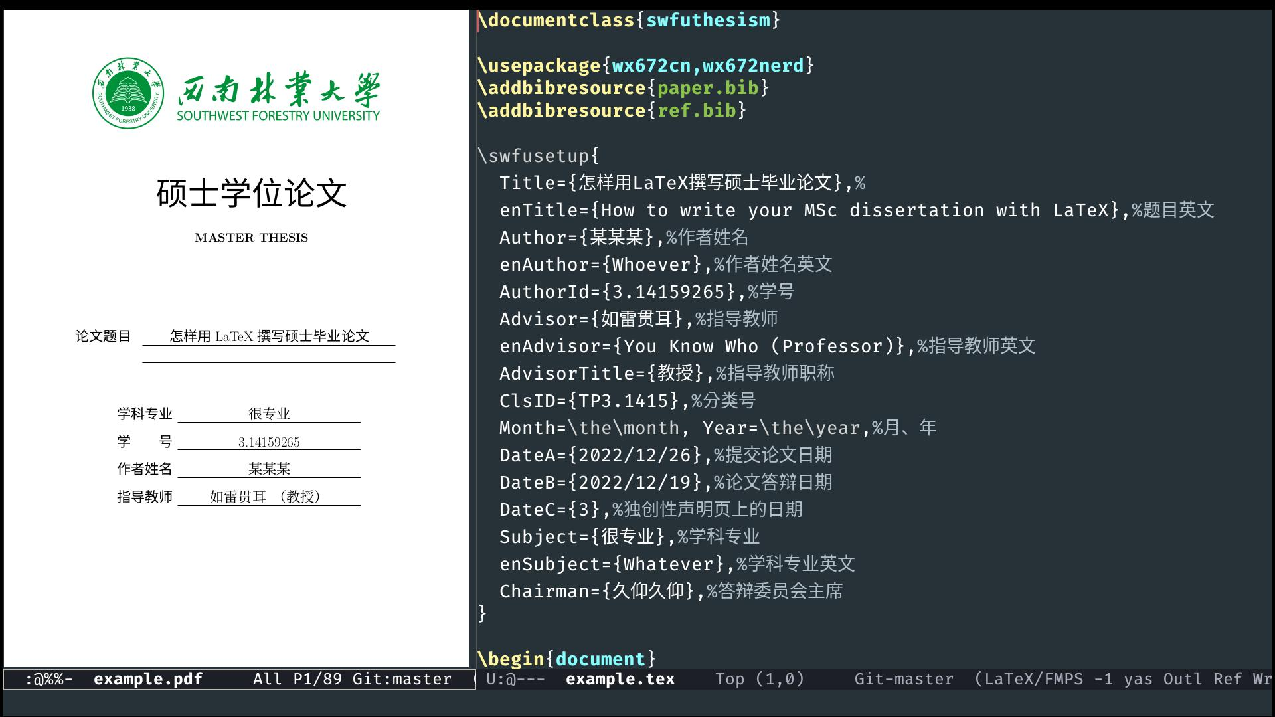
\includegraphics[width=.9\textwidth]{screenshot}
    \caption{在Emacs中编辑、预览论文\label{fig:screenshot}}  
\end{figure}

附录\ref{app:pkg}中列出了我的Debian系统上安装的与写论文相关的所有软件包,当然,清单里的
东西并非都是必需。其实,除了中文字体之外,其它的一切,你都可以根据自己的偏好来选择。如果你
打算用英文写论文的话,那么连中文字体都可以省略了。不管怎么说,上面提到的都是我个人的偏好,
本教程也将以此为基础,逐步展开。

至于如何安装、配置好这样一个工作环境,如果你是本校的学生,那么当然可以
直截找我帮忙。如果找不到我,那么你可以参考一下我曾经写过的一个简单的%
《Debian安装指导》\footnote{%
  \url{https://github.com/wx672/lecture-notes/blob/master/linux/tutorials/install/install.html}},应该能对你有点帮助的。

%%% Local Variables:
%%% mode: latex
%%% TeX-master: "../tutorial"
%%% End:
